%%%%%%%%%%%%%%%%%%%%%%%%%%%%%%%%%%%%%%%%%
% Short Sectioned Assignment LaTeX Template Version 1.0 (5/5/12)
% This template has been downloaded from: http://www.LaTeXTemplates.com
% Original author:  Frits Wenneker (http://www.howtotex.com)
% License: CC BY-NC-SA 3.0 (http://creativecommons.org/licenses/by-nc-sa/3.0/)
%%%%%%%%%%%%%%%%%%%%%%%%%%%%%%%%%%%%%%%%%

%----------------------------------------------------------------------------------------
%	PACKAGES AND OTHER DOCUMENT CONFIGURATIONS
%----------------------------------------------------------------------------------------

\documentclass[paper=a4, fontsize=11pt]{scrartcl} % A4 paper and 11pt font size

% ---- Entrada y salida de texto -----

\usepackage[T1]{fontenc} % Use 8-bit encoding that has 256 glyphs
\usepackage[utf8]{inputenc}
%\usepackage{fourier} % Use the Adobe Utopia font for the document - comment this line to return to the LaTeX default

% ---- Idioma --------

\usepackage[spanish, es-tabla]{babel} % Selecciona el español para palabras introducidas automáticamente, p.ej. "septiembre" en la fecha y especifica que se use la palabra Tabla en vez de Cuadro

% ---- Otros paquetes ----
\usepackage{alltt}
\usepackage{hyperref}
\usepackage{url} % ,href} %para incluir URLs e hipervínculos dentro del texto (aunque hay que instalar href)
\usepackage{amsmath,amsfonts,amsthm} % Math packages
%\usepackage{graphics,graphicx, floatrow} %para incluir imágenes y notas en las imágenes
\usepackage{graphics,graphicx, float} %para incluir imágenes y colocarlas

\usepackage{cite}
\usepackage{listings}
\usepackage{xcolor}

% Para hacer tablas comlejas
%\usepackage{multirow}
%\usepackage{threeparttable}

%\usepackage{sectsty} % Allows customizing section commands
%\allsectionsfont{\centering \normalfont\scshape} % Make all sections centered, the default font and small caps

\usepackage{fancyhdr} % Custom headers and footers

\setcounter{secnumdepth}{0}
\pagestyle{fancyplain} % Makes all pages in the document conform to the custom headers and footers
\fancyhead{} % No page header - if you want one, create it in the same way as the footers below
\fancyfoot[L]{} % Empty left footer
\fancyfoot[C]{} % Empty center footer
\fancyfoot[R]{\thepage} % Page numbering for right footer
\renewcommand{\headrulewidth}{0pt} % Remove header underlines
\renewcommand{\footrulewidth}{0pt} % Remove footer underlines
\setlength{\headheight}{13.6pt} % Customize the height of the header

\numberwithin{equation}{section} % Number equations within sections (i.e. 1.1, 1.2, 2.1, 2.2 instead of 1, 2, 3, 4)
\numberwithin{figure}{section} % Number figures within sections (i.e. 1.1, 1.2, 2.1, 2.2 instead of 1, 2, 3, 4)
\numberwithin{table}{section} % Number tables within sections (i.e. 1.1, 1.2, 2.1, 2.2 instead of 1, 2, 3, 4)

\setlength\parindent{0pt} % Removes all indentation from paragraphs - comment this line for an assignment with lots of text

\newcommand{\horrule}[1]{\rule{\linewidth}{#1}} % Create horizontal rule command with 1 argument of height


%----------------------------------------------------------------------------------------
%	TÍTULO Y DATOS DEL ALUMNO
%----------------------------------------------------------------------------------------

\title{	
\normalfont \normalsize 
\textsc{\textbf{Ingeniería de Servidores (2016-2017)} \\ Grado en Ingeniería Informática \\ Unisversidad de Granada} \\ [25pt] % Your university, school and/or department name(s)
\horrule{0.5pt} \\[0.4cm] % Thin top horizontal rule
\huge Memoria Práctica 1 \\ % The assignment title
\horrule{2pt} \\[0.5cm] % Thick bottom horizontal rule
}

\author{José Álvaro Garrido López} % Nombre y apellidos

\date{\normalsize\today} % Incluye la fecha actual

%----------------------------------------------------------------------------------------
% DOCUMENTO
%----------------------------------------------------------------------------------------

\begin{document}

\maketitle % Muestra el Título

\newpage %inserta un salto de página

\tableofcontents % para generar el índice de contenidos

\listoffigures

\listoftables

\newpage

\newpage
%----------------------------------------------------------------------------------------
%	Cuestión 1
%----------------------------------------------------------------------------------------

\section{Cuestión 1. ¿Qué modos y/o tipos de $"$virtualización$"$ existen? (no más de tres párrafos)}

Según un documento de la página oficial de \textbf{Oracle} [1],
la \textbf{virtualización} es la capacidad de ejecutar en un mismo hardware múltiples máquinas virtuales.
También apunta que de esta forma se pueden instalar varios sistemas operativos y por supuesto ejecutarlos de forma simultánea e independiente, cada uno en su propio entorno y con sin mermar el rendimiento de ambos en la medida de lo posible.
"Cada máquina virtual tiene su propia CPU virtual, interfaces de conexión virtuales, almacenamiento y sistema operativo."

En cuanto a \textbf{Intel}, como podemos comprobar en [2], asegura la existencia de al menos tres tipos de virtualización:
\newline\newline
- \textbf{Virtualización de CPU:} Este tipo de virtualización permite ejecutar software en la máquina virtual sin problemas de rendimiento o compatibilidad, lo cual hace posible incluso que se utilice la virtualización anidada.

- \textbf{Virtualización de memoria:} Las características de la virtualización de memoria permiten principalmente monitorizar el uso de la memoria en una máquina virtual base, mejorar la tolerancia a fallos y reforzar la seguridad.

- \textbf{Virtualización E/S:} Se utiliza para asignar funciones a las máquinas virtuales, con el fin de mejorar y facilitar la descarga y procesamiento de paquetes a los adaptadores de red. También es útil para mejorar el procesamiento de E/S. 
A modo de anotación personal, según lo leído en esta página oficial de \textbf{Intel}, entiendo que podrían utilizar procesadores virtuales que se encarguen de esperar la E/S, y de esta forma no ocuparíamos un core físico en realizar esta tarea, el cual puede continuar ejecutando instrucciones que aprovechan mejor la capacidad de procesamiento de un core.

%------------------------------------------------


%----------------------------------------------------------------------------------------
%	Cuestión 2
%----------------------------------------------------------------------------------------

\section{Cuestión 2. Muestre los precios y características de varios proveedores de VPS (Virtual Private Server) y compare con el precio de servidores dedicados (administrados y no administrados). Comente diferencias.}

Host Europe [22], tiene 3 propuestas para VPS, se muestran en la Tabla 2.1 y en la Tabla 2.2. Son administrador gratuitamente.

\begin{table}[h]
\begin{tabular}{l | c | c | c }
 & Alpha $\alpha$ & Delta $\delta$ & Omega $\omega$ \\
 \hline
 RAM garantizada& 2 GB & 4 GB & 8 GB \\
 RAM dinámica & 4 GB & 8 GB & 16 GB \\
 Espacio en disco & 200 GB SATA & 400 GB SATA & 600 GB SATA \\
 Precio & 9,99 euros/mes & 14,99 euros/mes &  19,99 euros/mes \\
 \end{tabular}
 \caption{Host Europe SATA}
 \label{hevpssata}
 \end{table}
 
Si seleccionamos SSDs el precio varía:
 
\begin{table}[h]
\begin{tabular}{l | c | c | c }
 & Alpha $\alpha$ & Delta $\delta$ & Omega $\omega$ \\
 \hline
 Espacio en disco & 100 GB SSD & 200 GB SSD & 300 GB SSD \\
 Precio & 9,99 euros/mes & 14,99 euros/mes &  19,99 euros/mes \\
 \end{tabular}
 \caption{Host Europe SSD}
 \label{hevpsssd}
 \end{table}
 
Servidores dedicados:

Los servidores de Host Europe dedicados son no administrados, pero se puede contratar al equipo de Host Europe para ello (no aparece información sobre el precio). En la Tabla 2.3 se exponen los modelos que se ofrecen:

\begin{table}[h]
\begin{tabular}{l | c | c | c}
 & ProServer X7 & ProServer X8 & ProServer X8i \\
\hline
RAM & 32 GB DDR3 & 32 GB DDR3 & 32 GB DDR3 \\
Discos duros & 2 $\times$ 2 TB o 2 $\times$ 256 GB & 2 $\times$ 2 TB o 2 $\times$ 256 GB & 2 $\times$ 3 TB o 2 $\times$ 512 GB \\
Procesadores
Precio & 39,99 euros/mes & 49,99 euros/mes & 59,99 euros/mes \\
\end{tabular}
\caption{Host Europe dedicados}
\label{heselin}
\end{table}

En cuanto al sistema operativo, se nos da a elegir entre Windows o Linux y todos disponen de software RAID1.

Es evidente que depende de lo que necesitemos, es mejor la utilización de un VPS o un dedicado, ya que el dedicado es cierto que nos ofrece unas prestaciones que no prometen mucho, pero a cambio de un precio muy bajo. Sin embargo, los servidores dedicados nos aseguran un gran rendimiento, debido al procesador, la cantidad de RAM, espacio en disco, etc, pero requieren de una inversión mayor.


%----------------------------------------------------------------------------------------
%	Cuestión 3
%----------------------------------------------------------------------------------------

\section{Cuestión 3. a) Enumere y explique brevemente al menos tres de las innovaciones en Windows Server 2016 y 2012 R2 respecto a 2008R2. b) ¿Qué es Windows Server 2016 nano?}

\subsection{a)} Comparando primero \textbf{Windows Server 2012 R2} con respecto a \textbf{2008 R2}, según \textbf{Microsoft}, en [3], \textbf{Windows Server 2012 R2}:

- Consigue \textbf{mejorar el rendimiento} de su anterior versión con una mayor capacidad para abordar cargas de trabajo de gran escala, más enfocado a servidores de altas prestaciones
- Incluye nuevas herramientas para gestionar redes, almacenamiento, \textbf{virtualización} y más
- La característica más destacable, es que \textbf{Windows Server 2012 R2} es mucho más escalable que el \textbf{2008 R2}, en este fragmento de tabla extraída de [3], la Tabla 3.1, podemos ver algunas de las mejoras en cuanto a escalabilidad:

\begin{table}[H]
\centering
\begin{tabular}{|c|c|c|}
\hline
\textbf{ Característica} & \textbf{Windows Server 2008 R2} & \textbf{Windows Server 2012 R2} \\
\hline
Procesadores lógicos & 64 & 320 \\
Procesadores virtuales & 512 & 2048 \\
Memoria física & 1 TB & 4 TB \\
Máquinas virtuales activas & 384 & 1024 \\
\hline
\end{tabular}  
\caption{Windows 2008 R2 vs Windows 2012 R2} \label{tab:ws2008vsws2012}
\end{table}

En cuanto a las mejoras de Windows Server 2016 frente a Windows Server 2012 R2, en [4] Microsoft nos explica las más relevantes:

Las máquinas tanto físicas como virtuales ven mejorado su rendimiento sobre todo gracias a las mejoras realizadas en Hyper-V, el software de virtualización de Windows [5]:\newline

-  \textbf{Arranque seguro Linux:} Permite iniciar con la opción de arranque seguro sistemas operativos Linux en máquinas virtuales (Ubuntu, SUSE, RedHat y CentOS)

- \textbf{Soporte para más memoria y procesadores para hosts de Hyper-V:} Esto permite la administración de bases de datos grandes en memoria para el procesamiento de las mismas. Es interesante saber que se ha conseguido un rendimiento en torno al 95\% de un servidor virtual dentro de uno físico

- \textbf{Virtualización anidada:} Permite utilizar una máquina virtual como host Hyper-V de otras máquinas virtuales dentro de la misma. Es útil para desarrollar y testear

\subsection{b)}

Según podemos comprobar en la página oficial de Microsoft [4], Windows  Server 2016 Nano es una opción de instalación de este sistema operativo. Se trata de un sistema operativo que se administra de forma remota. Está pensado y optimizado para pequeños servidores en la nube y centros de procesamiento de datos privados, ya que es más ligero, ocupa menos espacio, es más rápido, se configura y se instala más fácilmente.

%----------------------------------------------------------------------------------------


%----------------------------------------------------------------------------------------
%	Cuestión 4
%----------------------------------------------------------------------------------------

\section{Cuestión 4. ¿Qué son los productos MAAS y Landscape ofrecidos por Canonical (la empresa que desarrolla Ubuntu?}

Canonical nos proporciona documentación sobre \textbf{MAAS} (Metal As A Service) en una sección de la página web oficial de Ubuntu [6], donde se nos explica que \textbf{MAAS} es una herramienta que permite gestionar en la nube los servidores físicos como si fueran máquinas virtuales. De esta forma, no es necesario administrar cada uno de los servidores físicos de forma individual, sino que lo podemos hacer simultáneamente con todos a través de Internet.

Funciona de la siguiente forma: Hay que especificar los servidores que se desean administrar y \textbf{MAAS} los ejecuta y les pasa un test de hardware, después del mismo están operativos para ser gestionados desde la nube.\newline

En [7], Canonical nos explica que \textbf{Landscape} es una herramienta para monitorizar, gestionar y ejecutar servidores de Ubuntu.
Para ello, está provisto de herramientas que facilitan dichos objetivos, como la automatización de tareas que se deben ejecutar de forma diaria, avisos para actualizar los servidores, parches de seguridad, creación de repositorios software y la capacidad de gestionar hasta 40000 máquinas con esta interfaz.

%----------------------------------------------------------------------------------------

%----------------------------------------------------------------------------------------
%	Cuestión 5
%----------------------------------------------------------------------------------------

\section{Cuestión 5. ¿Qué relación tiene esta distribución con Red Hat y con el
proyecto Fedora?}

Según [8], \textbf{Red Hat} y el proyecto \textbf{CentOS} están desarrollando un nuevo sistema operativo \textbf{CentOS}, con el fin de "promover el desarrollo y adopción de una nueva generación de proyectos de software libre", como se indica en la página web de \textbf{Red Hat}.

\textbf{Red Hat} pretende colaborar con sus recursos y experiencia para apoyar a los usuarios de \textbf{CentOS} y desarrollar nuevas tecnologías en virtualización, software en la nube y otros proyectos.

En cuanto a la relación con el proyecto \textbf{Fedora}, en [9], \textbf{Red Hat} explica la relación existente entre su empresa y \textbf{Fedora}.
Las distribuciones de \textbf{Fedora Linux} y \textbf{Red Hat Enterprise Linux} son de código abierto, la primera desarrollada por la \textbf{comunidad Fedora} y la segunda por \textbf{Red Hat}.
\textbf{Red Hat} y \textbf{Fedora} se benefician mutuamente, pues \textbf{Red Hat} puede aprovecharse de la gran capacidad de \textbf{Fedora} para desarrollar e implementar la tecnología más reciente, y \textbf{Fedora} del patrocinio que la empresa le proporciona.

%----------------------------------------------------------------------------------------

%----------------------------------------------------------------------------------------
%	Cuestión 6
%----------------------------------------------------------------------------------------

\section{Cuestión 6: ¿Qué diferencias hay entre RAID mediante SW y mediante HW?}

Según la documentación de \textbf{Red Hat} [20], los sistemas basados en hardware gestionan el \textbf{RAID} independientemente desde el host. Para esta forma de implementación de un \textbf{RAID}, son necesarios dispositivos inteligentes que gestionen los controladores de los discos, estos son bastante caros pero muy eficientes. En muchos casos permiten la desconexión en caliente de las unidades de disco. No utilizan al procesador para gestionar el \textbf{RAID}, lo cual lo desocupa de este tipo de tareas para centrarse en otras, y es posible que se aprecie en el rendimiento de forma positiva.

El \textbf{RAID} por software implementa los diferentes niveles del \textbf{RAID} en el código del disco en el kernel. Es una forma más barata que la implementación de \textbf{RAID} por hardware, ya que no se necesitan tarjetas controladoras de discos o chasis para desconexión en caliente. Gracias a la capacidad de procesamiento de los procesadores de hoy en día, puede darse el caso en el que el \textbf{RAID} por software supere al \textbf{RAID} por hardware en rendimiento.
El dispositivo MD (que hemos tenido que crear siguiendo el guión de la práctica 1) es una solución \textbf{RAID} software.

%----------------------------------------------------------------------------------------

%----------------------------------------------------------------------------------------
%	Cuestión 7
%----------------------------------------------------------------------------------------

\section{Cuestión 7: a) ¿Qué es LVM? b)¿Qué ventaja tiene para un servidor de
gama baja? c) Si va a tener un servidor web, ¿le daría un tamaño grande o
pequeño a /var?}

\subsection{a)}
Según la wiki de \textbf{Archlinux}, [23], \textbf{LVM} es un gestor de volúmenes lógicos para el kernel de \textbf{Linux}, que sirve para gestionar dispositivos de almacenamiento masivo y unidades de disco.

\subsection{b)}
En la página web de \textbf{The Linux Documentation Project} [18], existe una sección que explica esto:

Es común que los usuarios no muy experimentados en Linux sufran dudas a la hora de definir el espacio de cada una de las particiones que desea crear. Sin embargo, LVM permite que todas las particiones sean creadas en el mismo volumen físico de la unidad de almacenamiento, dentro de esta se pueden crear los volúmenes lógicos que se quieran. Esto permite que si alguno de los volúmenes lógicos se queda sin espacio, podemos reconfigurar el espacio dedicado a cada una de ellas.

\subsection{c)}
Según [19], donde se explican los directorios que contiene \textit{/var,} uno de ellos es \textit{/var/cache/www}.
Si vamos a crear un servidor web, dicho directorio será uno de los más importantes y de los que más espacio necesitará, porque será donde tendremos la mayor parte de la información, así que le daría un tamaño grande.

%----------------------------------------------------------------------------------------

%----------------------------------------------------------------------------------------
%	Cuestión 8
%----------------------------------------------------------------------------------------

\section{Cuestión 8. ¿Debemos cifrar también el volumen que contiene el espacio
para swap? ¿y el volumen en el que montaremos /boot?}

En la wiki de \textbf{Arch Linux}, [23], aparece información al respecto: debemos cifrar el volumen que contiene el área de intercambio, ya que es un volumen de la unidad de almacenamiento que se utiliza para cargar los programas cuando la memoria RAM está llena, por lo cual puede haber información que no nos interese que pueda ser interceptada.
Sin embargo el volumen en el que montamos /boot no es necesario cifrarlo ya que solo contiene información para el arranque de la máquina, además si lo cifráramos, no podríamos acceder al sistema operativo a través de esta partición de forma directa, ya que es la que va a contener las instrucciones a bajo nivel sobre cómo acceder a todas las particiones.

%----------------------------------------------------------------------------------------

%----------------------------------------------------------------------------------------
%	Cuestión 9
%----------------------------------------------------------------------------------------

\section{Cuestión 9. a) Imagine que tiene un disco híbrido con tecnología SSD. ¿Qué puntos de montaje ubicaría en este? b) Justifique qué tipo de sistema de archivos usaría para tener un servidor de streaming}

\subsection{a)}
Ubicaría /home y /swap en el HDD y /boot y / en el SSD, ya que en /boot está la información necesaria para iniciar la máquina, y en / el sistema operativo y algunos programas que se instalen.
En primera instancia no pondría /swap en el SSD por el increíble desgaste que el mismo sufriría, pues los SSD, aunque tengan un mayor rendimiento en escritura y lectura de datos tienen una menor vida útil, ubicando /swap en el SSD sufriríamos un desgaste prematuro del mismo, y a no ser que nos importe mucho el rendimiento en el caso en concreto o que disupusiéramos de un SSD con endurecimiento de escritura o lectura, no lo haría. En definitiva, depende mucho del caso concreto en el que nos situemos, pero por lo general haría lo descrito anteriormente.
Para responder a esta pregunta he utilizado como fuente los conocimientos que he adquirido en la rama de \textbf{Ingeniería de Computadores}.

\subsection{b)}
En la wiki de \textbf{Ubuntu} se explican diversos sistemas de archivos para \textbf{Linux}, entre ellos, \textbf{ZFS}, en [21], donde se exponen las principales características de este robusto sistema de archivos desarrollado por \textbf{Sun Microsystems}. Lo que me ha llevado a elegir este sistema de archivos es su capacidad para comprimir los archivos que tengan cierto tamaño (a partir del que se consideran grandes) de forma automática, lo cual sería beneficioso para manejar las grandes cantidades de información de un servidor de streaming.
También he elegido este sistema de archivos por su capacidad para aplicar algoritmos automáticamente cuando se está realizando un streaming, asegurando un gran rendimiento.

%----------------------------------------------------------------------------------------

%----------------------------------------------------------------------------------------
%	Cuestión 10
%----------------------------------------------------------------------------------------

\section{Cuestión 10. Muestre cómo ha quedado el disco particionado una vez el sistema está instalado y ha iniciado sesión. (comando lsblk)}

Como podemos comprobar en la Figura 10.1, el particionado queda como un $"$espejo$"$ del segundo disco sobre el primero, objetivo que queríamos cumplir al configurar el \textbf{RAID1}. Cada disco tiene los cuatro volúmenes lógicos encriptados con \textbf{LVM} en la configuración que previamente realizamos, el disco "hogar", el "swap", el "arranq" y el "raiz", todos cifrados a excepción del arranque.

\begin{figure}[H] %con el [H] le obligamos a situar aquí la figura
\centering
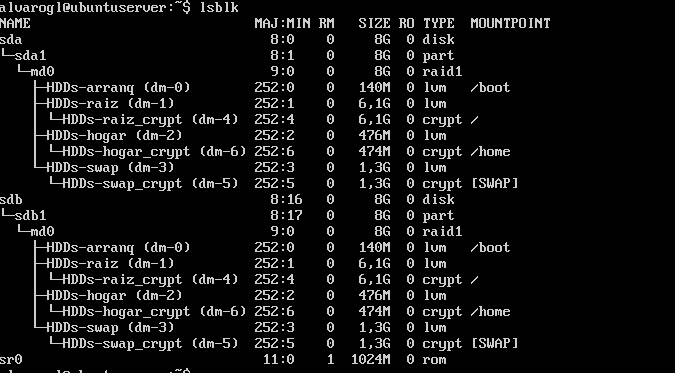
\includegraphics[scale=0.8]{cuestion10-lsblk.PNG}  %el parámetro scale permite agrandar o achicar la imagen. En el nombre de archivo puede especificar directorios
\caption{Particionado del disco después de la instalación del sistema (orden lsblk)} \label{fig:figura1}
\end{figure}

%----------------------------------------------------------------------------------------


%----------------------------------------------------------------------------------------
%	Cuestión 11
%----------------------------------------------------------------------------------------

\section{Cuestión 11. a) ¿Cómo ha hecho el disco 2 $"$arrancable$"$? b) ¿Qué hace el comando grub-install?}

\subsection{a)}
Siguiendo la instalación de \textbf{Ubuntu Server 14} en el guión de la \textbf{práctica 1 de Ingeniería de Servidores}, y después de configurar las particiones y el \textbf{RAID}, se nos pregunta de forma automática si deseamos instalar el cargador de arranque sobre el disco 1 (sda), esto ejecuta el comando \textbf{\textit{grub-install /dev/sda}}, lo cual podemos hacer de forma manual también con el disco 2 (sdb), con el comando \textbf{\textit{grub-install /dev/sdb}}.
En la Figura 11.1 se ilustra cómo podríamos encontrar la unidad de almacenamiento donde deseamos instalar el GRUB, ya que la orden ejecutada (\textbf{\textit{ls /dev/}}) nos muestra todos los dispositivos conectados y en la Figura 11.2, la ejecución de la orden grub-install sobre la misma

\begin{figure}[H] %con el [H] le obligamos a situar aquí la figura
\centering
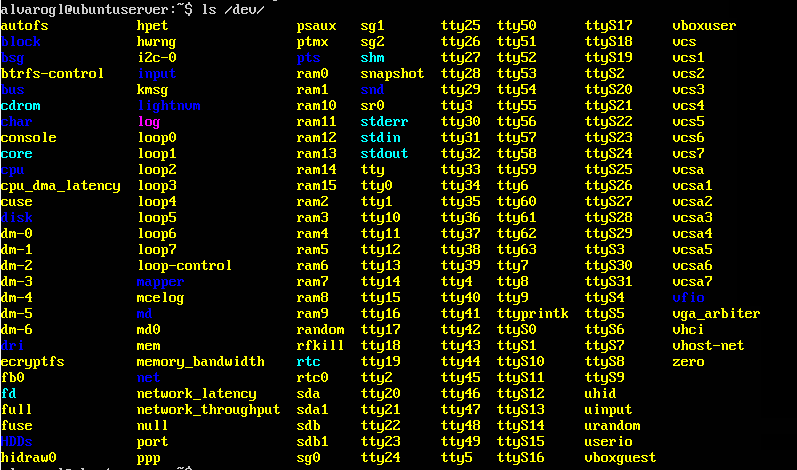
\includegraphics[scale=0.8]{cuestion11-unidades.PNG}  %el parámetro scale permite agrandar o achicar la imagen. En el nombre de archivo puede especificar directorios
\caption{Búsqueda de unidad de almacenamiento} \label{fig:figura1}
\end{figure}

\begin{figure}[H] %con el [H] le obligamos a situar aquí la figura
\centering
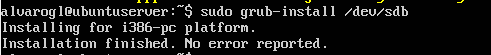
\includegraphics[scale=0.8]{cuestion11-grub-install.PNG}  %el parámetro scale permite agrandar o achicar la imagen. En el nombre de archivo puede especificar directorios
\caption{Ejecución del comando \textbf{\textit{grub-install}} sobre el disco 2} \label{fig:figura1}
\end{figure}

\subsection{b)}
Según el manual de instalación del \textbf{GRUB} de la página oficial de \textbf{GNU} [10], el comando grub-install instala el gestor de arranque múltiple \textbf{GRUB} en el \textbf{MBR} (Master Boot Record) del disco que indiquemos como argumento. El argumento debe ser un archivo de dispositivo. Los ficheros de dispositivos en \textbf{Linux} se encuentran en '/dev'. Si nuestro fichero de dispositivo se llama 'hda' para instalar en dicho dispositivo el \textbf{GRUB} debemos ejecutar el comando:\newline

\textbf{\textit{grub-install /dev/hda}}

%----------------------------------------------------------------------------------------


%----------------------------------------------------------------------------------------
%	Cuestión Opcional 1
%----------------------------------------------------------------------------------------

\section{Cuestión Opcional 1. Muestre (con capturas de pantalla) cómo ha comprobado que el RAID1 funciona}

En mi caso, he utilizado la forma explicada en el guión de la práctica 1 de \textbf{Ingeniería de Servidores}:
He creado un archivo 'test\_raid', como se muestra en la Figura 12.1, he desenchufado el disco 2 (Figura 12.2), y he probado a iniciar el sistema operativo, el cual no ha iniciado el shell de 'initramfs' después de unos segundos, shell que, según \textbf{Ubuntu}, en [11], es una herramienta capaz de arrancar sistemas operativos. Según la wiki de kernel.org [12], podemos iniciar un \textbf{RAID} desde el shell de initramfs utilizando la orden (Figura 12.3).

\textbf{textit{mdadm --run /dev/md0}}

Una vez que hemos conseguido arrancar \textbf{Ubuntu}, comprobamos que el archivo que habíamos creado efectivamente existe. El \textbf{RAID} funciona (Figura 12.4).

\begin{figure}[H] %con el [H] le obligamos a situar aquí la figura
\centering
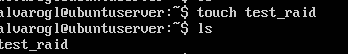
\includegraphics[scale=0.8]{cuestionopc1-creamosarchivohome.PNG}  %el parámetro scale permite agrandar o achicar la imagen. En el nombre de archivo puede especificar directorios
\caption{Creación del archivo en /home} \label{fig:figura1}
\end{figure}

\begin{figure}[H] %con el [H] le obligamos a situar aquí la figura
\centering
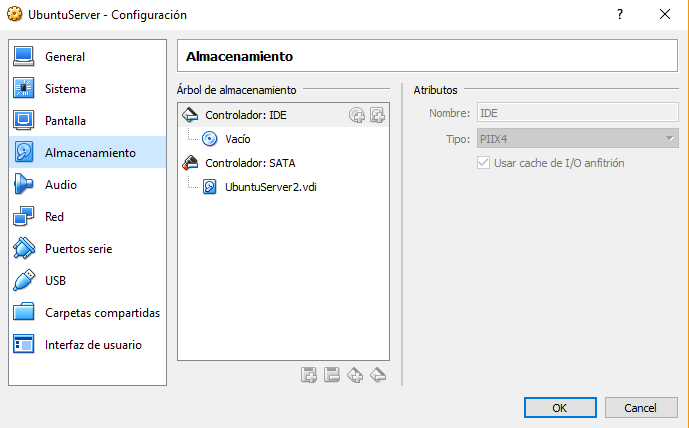
\includegraphics[scale=0.8]{cuestionopc1-desenchufamosdisco1.PNG}  %el parámetro scale permite agrandar o achicar la imagen. En el nombre de archivo puede especificar directorios
\caption{Creación del archivo en /home} \label{fig:figura1}
\end{figure}

\begin{figure}[H] %con el [H] le obligamos a situar aquí la figura
\centering
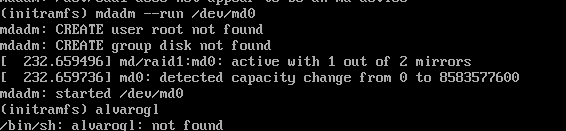
\includegraphics[scale=0.8]{cuestionopc1-mdadmconnombre.PNG}  %el parámetro scale permite agrandar o achicar la imagen. En el nombre de archivo puede especificar directorios
\caption{Ejecución de \textbf{\textit{mdadm}}} \label{fig:figura1}
\end{figure}

\begin{figure}[H] %con el [H] le obligamos a situar aquí la figura
\centering
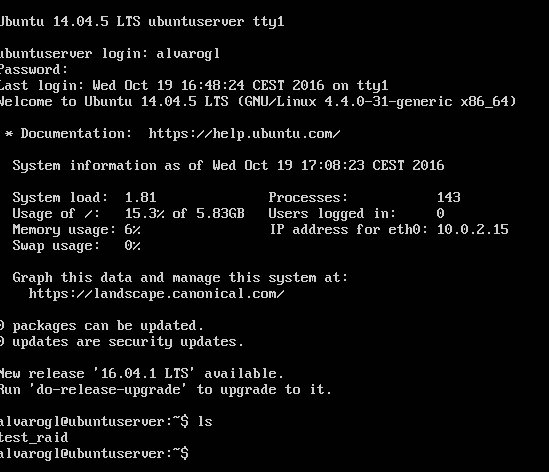
\includegraphics[scale=0.8]{cuestionopc1-comprobacionraidcorrecta.PNG}  %el parámetro scale permite agrandar o achicar la imagen. En el nombre de archivo puede especificar directorios
\caption{Comprobación de que \textbf{RAID} funciona} \label{fig:figura1}
\end{figure}

%----------------------------------------------------------------------------------------

%----------------------------------------------------------------------------------------
%	Cuestión 12
%----------------------------------------------------------------------------------------

\section{Cuestión 12. ¿Qué diferencia hay entre Standard y Datacenter?}

Como podemos ver en la página web oficial de Microsoft, en [14], la versión Standard está desarrollada para clientes que no necesitan demasiadas instancias virtuales de Windows Server, ya que solo permite ejecutar dos de ellas, las cuales proporcionan las mismas características que la versión Datacenter (excepto el número de instancias virtuales).
Datacenter sin embargo, no limita el número de instancias de Windows Server por licencia. De esta forma, permite el crecimiento del entorno virtual tanto como se desee (mientras el hardware lo soporte).

Según [15], las diferencias no solo radican en las características, sino por supuesto, en el precio, ya que la licencia de Windows Server 2012 R2 Datacenter cuesta 6155 dólares estadounidenses y la licencia Standard es más asequible, costando 882 dólares estadounidenses.

%----------------------------------------------------------------------------------------

%----------------------------------------------------------------------------------------
%	Cuestión 13
%----------------------------------------------------------------------------------------

\section{Cuestión 13. ¿Continúe usted con el proceso de definición de RAID1 para los dos discos de 50 MiB que ha creado. Muestre el proceso con capturas de pantalla.}

Según el soporte de \textbf{Microsoft}, en [13], para reflejar las particiones (\textbf{RAID1}), debemos acceder a \textbf{Herramientas administrativas} en \textbf{Inicio}, y después a \textbf{Administración de equipos}.

En \textbf{Almacenamiento} y \textbf{Administración de discos} nos aparece la lista de discos del equipo. Hacemos click derecho en uno de los discos nuevos de 50 MiB y le damos a \textbf{Nuevo volumen reflejado}, seguimos el \textit{Wizard} y terminamos el proceso. (Figura 14.1).
En la Figura 14.2 se muestra cómo quedan los discos después de esta configuración.

\begin{figure}[H] %con el [H] le obligamos a situar aquí la figura
\centering
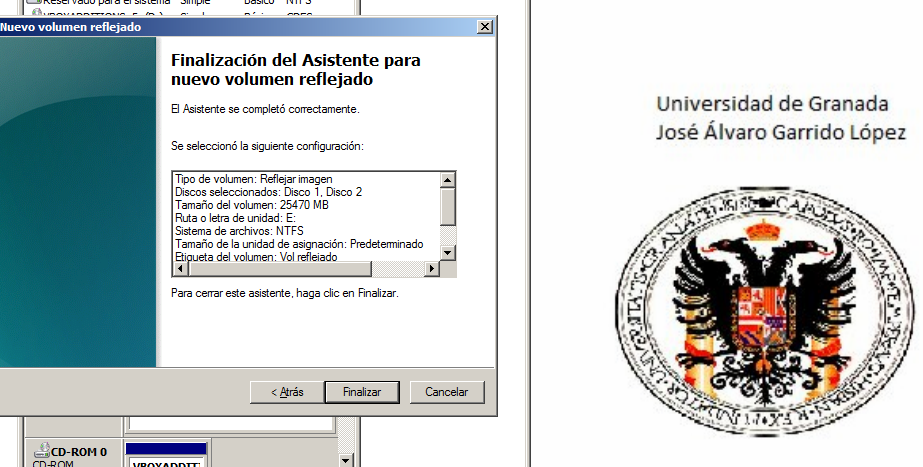
\includegraphics[scale=0.65]{cuestion13-RAID1.PNG}  %el parámetro scale permite agrandar o achicar la imagen. En el nombre de archivo puede especificar directorios
\caption{\textit{Wizard} para configurar \textbf{RAID1}} \label{fig:figura1}
\end{figure}

\begin{figure}[H] %con el [H] le obligamos a situar aquí la figura
\centering
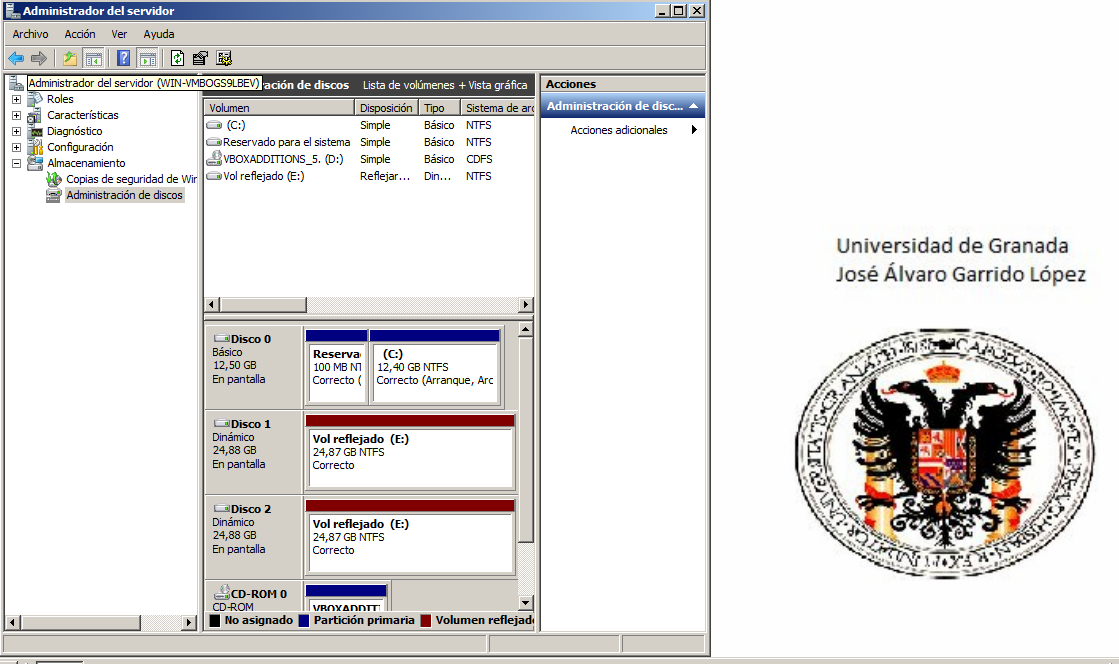
\includegraphics[scale=0.5]{cuestion13-VolReflejados.PNG}  %el parámetro scale permite agrandar o achicar la imagen. En el nombre de archivo puede especificar directorios
\caption{\textbf{RAID1} configurada} \label{fig:figura1}
\end{figure}

%----------------------------------------------------------------------------------------

%----------------------------------------------------------------------------------------
%	Cuestión 14
%----------------------------------------------------------------------------------------

\section{Cuestión 14. Explique brevemente qué diferencias hay entre los tres tipos de conexión que permite el VMSW para las MVs: NAT, Host-only y Bridge.}

En el manual de \textbf{VirtualBox}, [16], se explican, entre otros, los tres tipos de conexión que se nos preguntan en el enunciado:

- \textbf{NAT}: \textbf{NAT} (Network Addres Translation) es la forma más simple de acceder a una red externa a una máquina virtual. Ni siquiera requiere de configuración en ninguno de los sistemas operativos (host o guest). Consiste en emular la conexión real que habría entre un computador que se conecta a un router.

- \textbf{Host-Only}: Es un modo de conexión que permite que las máquinas virtuales se intercambien información entre sí y el host como si estuvieran conectadas físicamente.

- \textbf{Bridge}: \textbf{VirtualBox} filtra la información del adaptador de red desde el sistema operativo host. De esta forma, el software puede interceptar información de la red física e introducir datos en ella, creando una interfaz de conexión entre el host y el sistema de la máquina virtual. El host puede enviar informacion al invitado a través de esa interfaz y recibir datos.

%------------------------------------------------

\section{Referencias}

[1] \textit{Documentación de Oracle acerca de la virtualización, } 
\url{https://docs.oracle.com/cd/E11081_01/doc/doc.21/e10898/intro.htm#CHDGBFIG}\newline
[2] \textit{Intel Virtualization Technology, }
\url{http://www.intel.la/content/www/xl/es/virtualization/virtualization-technology/intel-virtualization-technology.html}\newline
[3] \textit{Nuevas características de Windows Server 2012, }\newline
\url{https://www.microsoft.com/es-xl/server-cloud/products/windows-server-2012-r2/comparison.aspx}\newline
[4] \textit{Microsoft acerca de Windows 2016 Nano, }
\url{https://technet.microsoft.com/en-us/windows-server-docs/get-started/getting-started-with-nano-server}\newline
[5] \textit{Documentación acerca de Hyper-V en Windows Server 2016, }
\url{https://technet.microsoft.com/windows-server-docs/compute/hyper-v/what-s-new-in-hyper-v-on-windows}\newline
[6] \textit{Documentación de Ubuntu sobre MAAS, }
\url{https://maas.ubuntu.com/docs/}\newline
[7] \textit{Documentación de Canonical sobre Landscape, }
\url{https://landscape.canonical.com/}\newline
[8] \textit{Relación de Red Hat con CentOS, }
\url{https://community.redhat.com/centos-faq/}\newline
[9] \textit{Relación entre Fedora y Red Hat, }
\url{https://www.redhat.com/es/technologies/linux-platforms/articles/relationship-between-fedora-and-rhel}\newline
[10] \textit{Documentación de GNU sobre instalación de GRUB, }
\url{https://www.gnu.org/software/grub/manual/html_node/Installing-GRUB-using-grub_002dinstall.html}\newline
[11] \textit{Manual de Ubuntu sobre initramfs, }
\url{http://manpages.ubuntu.com/manpages/precise/man7/casper.7.html}\newline
[12] \textit{Documentación de kernel.org sobre mdadm, }
\url{https://raid.wiki.kernel.org/index.php/RAID_setup#Mdadm_modes_of_operation}\newline
[13] \textit{Soporte de Microsoft sobre cómo reflejar la partición de sistema (RAID1), }
\url{https://support.microsoft.com/es-es/kb/323432}\newline
[14] \textit{Información de Microsoft acerca de las diferentes versiones de Windows Server 2012 R2, }
\url{https://www.microsoft.com/en-us/licensing/product-licensing/windows-server-2012-r2.aspx}\newline
[15] \textit{Documentación de Microsoft acerca del precio de las diferentes versiones de Windows Server 2012 R2, }
\url{https://www.microsoft.com/es-es/server-cloud/products/windows-server-2012-r2/purchasing.aspx}\newline
[16] \textit{Documentación de VirtualBox acerca de los tipos de conexiones que se pueden realizar en una MV, }
\url{https://www.virtualbox.org/manual/ch06.html}\newline
[17] \textit{Documentación de Arch Linux sobre LVM, }
\url{https://wiki.archlinux.org/index.php/LVM_(Espa%C3%B1ol)}\newline
[18] \textit{Documentación de TLDP sobre los beneficios de LVM, }
\url{http://www.tldp.org/HOWTO/LVM-HOWTO/benefitsoflvmsmall.html}\newline
[19] \textit{Documentación de TLDP sobre los sistemas de archivos, }
\url{http://www.tldp.org/LDP/Linux-Filesystem-Hierarchy/html/var.html}\newline
[20] \textit{Documentación de Red Hat sobre RAID, }
\url{https://access.redhat.com/documentation/en-US/Red_Hat_Enterprise_Linux/3/html/System_Administration_Guide/s1-raid-approaches.html}\newline
[21] \textit{Documentación de Ubuntu sobre ZFS, }
\url{https://wiki.ubuntu.com/ZFS}\newline
[22] \textit{Servidores Virtuales Privados, Host Europe, }
\url{https://www.hosteurope.es/servidores-virtuales?gclid=CISFnrOB_s8CFQw8Gwod2cgIfQ}\newline
[23] \textit{Wiki Arch Linux, }
\url{https://wiki.archlinux.org/index.php/Dm-crypt/Swap_encryption}


\end{document}